\subsection{Preprocessing Algorithms}
\begin{frame}{Preprocessing Algorithms}
    \begin{columns}[T] % contents are top vertically aligned
    \begin{column}[T]{5cm} % each column can also be its own environment
        \begin{itemize}
            \item<1-> Normalizing
            \begin{itemize}
                \item<2-> Scaling
                \item<2-> Shifting
                \item<3-> Resampling
            \end{itemize}
            \item<1-> Noise reduction
            \begin{itemize}
                \item<4-> Smoothing (e.g. moving average)
                \item<5-> Dot reduction
                \item<6-> Filtering (by distance, speed or angle)
                \item<8-> Stroke connection
            \end{itemize}
        \end{itemize}
    \end{column}
    \begin{column}[T]{6cm} % alternative top-align that's better for graphics
        \only<2>{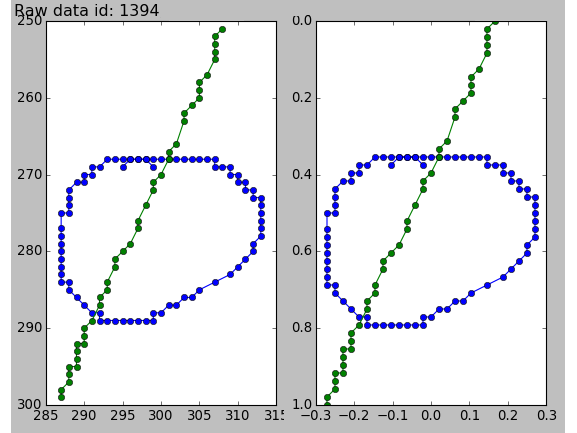
\includegraphics[width=6cm, keepaspectratio]{scale-and-shift.png}}
        \only<3>{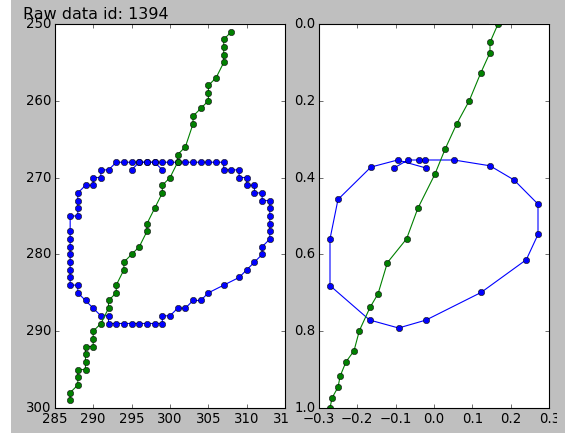
\includegraphics[width=6cm, keepaspectratio]{resampling.png}}
        \only<4>{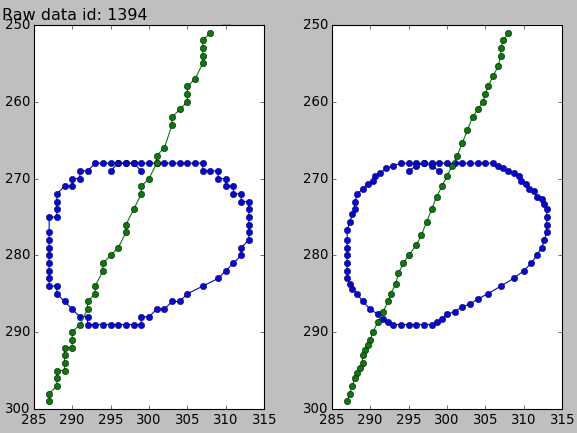
\includegraphics[width=6cm, keepaspectratio]{smooth-1-1-1.png}}
        \only<5>{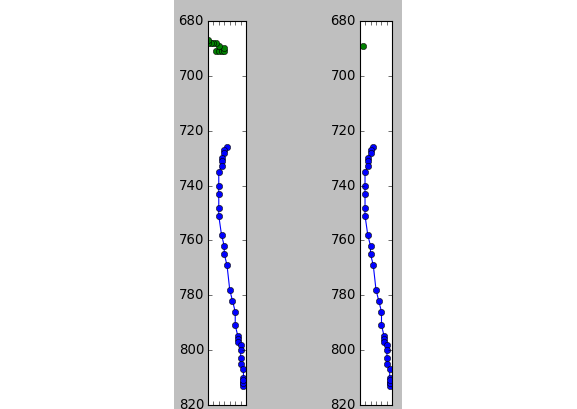
\includegraphics[width=6cm, keepaspectratio]{dot-reduction.png}}
        \only<6>{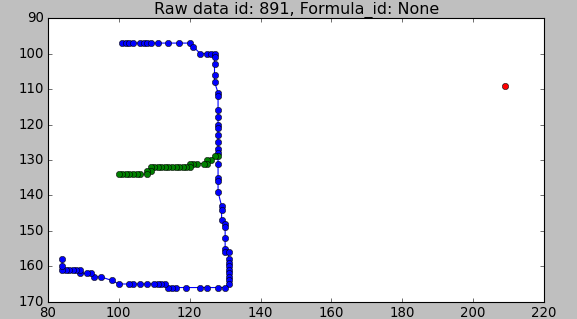
\includegraphics[width=6cm, keepaspectratio]{wildpoint-1.png}}
        \only<7>{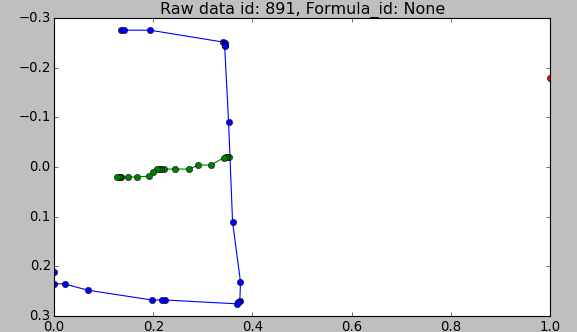
\includegraphics[width=6cm, keepaspectratio]{wildpoint-2.png}}
        \only<8>{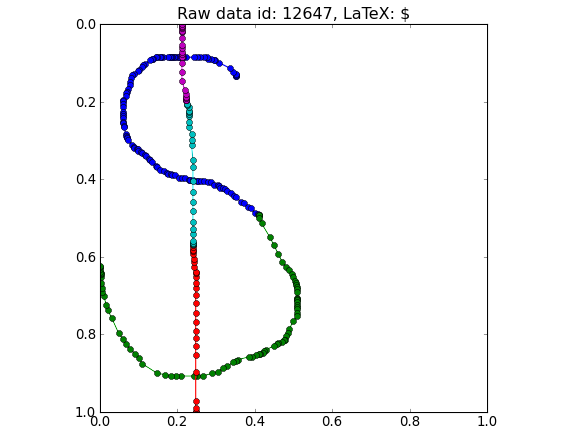
\includegraphics[width=6cm, keepaspectratio]{interrupted-stroke.png}}
    \end{column}
    \end{columns}
\end{frame}